\section{Systematic Uncertainties} \label{section:higgs_systematics}
All of the systematic uncertanties that come into play in this search, except for just one, are due to the potential effects of mismodeling Standard Model Higgs signal. In general we can identify several types of potential sources of problems in our model to correct for: shape of the SM Higgs Boson signal, the yield of the signal, and various experimental and theoretical uncertainties.
% Systematics uncertainties due to the mismodel of the signal have been taken into account in the signal extraction and discussed in this section.
% We distinguish between ``{\it shape}'' uncertainties, that affect the description of the peak in each category, ``{\it rate}'' uncertainties,
% that change the total number of Higgs events expected, and ``{\it category migration}'' uncertainties, that migrates events from one category to the other.

\subsection{Shape Uncertainties}
Nuisances responsible for the shape systematic uncertainties are used to address the potential mismatch of the expected signal peak in simulations with the data. There are two possible sources of such mismatch: the mean (the scale) of the signal mass distribution could be shifted or the width (the resolution) could be different.
\begin{itemize}
    \item {\bf Muon Scale}. Amounts up to 5\% of the muon momentum and the potential effect is to change the position of the Higgs signal with respect to its nominal value.
    \item {\bf Muon Resolution}, it amounts up to $10\%$. There are two important outcomes of this mismodeling. One is that the width of the signal can be different from the one sitting in the data. And second, as a consequence of the first, the wider the signal is, and noting how much more dominant the background is for our search, the easier it is for the background to ''eat'' our signal peak. In other words, some analytic functional forms are quite flexible in a way that they can contribute to the peaky structure for our signal, causing the improper modeling of our Standard Model Higgs signal and invalid extraction of Exlusion Limits.
\end{itemize}
The second point is of particular importance and will be addressed further in the next section~\ref{section:higgs_combination}.

\subsection{Category migration}
The following list of nuisances added to the model is primarily responsible for the migration of events across the categories. It has been verified within the statistical power of the MC that no major shape distortions are present.
\begin{itemize}
    \item {\bf Jet Energy Scale}, amounts up to 6\%. After applying the jet energy corrections, the energy scale of the jet is varied as a single nuisance parameter.
    % Due to VBF like classification this changes corresponds to yields variations, espetially  in the high sensitive categories, where it amounts up to $6\%$ in the  variations of the yields.
    Given that there are categories with the dominant VBF production process contribution, this nuisance can amount up to substantial yield variations, especially in the sensitive catogories. This uncertainty is the dominant experimental uncertainty in the measurement, i.e. the uncertainty with the largest impact on the parameter of interest among the ones listed.
    \item {\bf Jet Energy Resolution}, up to 1-2\%. The jet energy resolution can also induce category migration due to the non-linearly falling spectrum of the jet transverse momentum. It has a modest impact with respect to the scale and it amounts to up to few percent across the categories.
    \item {\bf Pileup Reweighting}, up to 1-2\%. Pileup Reweighting procedure uses the ''minimum bias'' cross section to extract the estimated amount of pileup in data. There are mainly 2 effects of PU: it can reduce the efficiency of the muon selection by an increasing of the amount of hadronic activity closed by, and it can promote random clusters of energy to identified jets.
    \item {\bf b jet efficiency}, up to 1\%. After correcting the efficiency of the b-jets passing the medium working point, uncertainties are assignied. Due to the fact that b-jets are vetoed on in the most sensitive categories, in order to suppress {$t\bar{t}$} contribution, this uncertainty yields to $\simeq 1\%$ variations.
    \item {\bf b jet fake rate}, up to 1\%. Similar to the above but corrects the efficiency of light-flavored jets to fake a b-jet ($\simeq 1\%$).
    \item {\bf MC f/r scale}, up to 6\%. Factorization and renormalization scale are varied up and down by a factor of $2$ in the MC using the MC weights present in the official production. The most extreme variations are excluded from this accounting ($r=0.5,f=2$ and $r=2,f=0.5$). This uncertainty yields up to $\simeq 6\%$ category migration and do not account for the sample total normalization.
    \item {\bf MC pdf}, up to 2-3\%. Parton Distribution Functions (PDFs) are varied using the NNPDF3.
\end{itemize}
% \begin{table}[h!]
%     \centering
%     \caption{Category migration for the jet energy scale uncertainty for ggH and qqH processes. Values yielding variations smaller than 1\% are suppressed. All the processes are present in the datacard. The two variations reported and separated by a slash corresponds to respectively the shift down and up in the jet energy scale; the nuisance parameter takes into account this correlation scheme when will be profiled.}
%     \label{tab:jes}
%     \resizebox{\columnwidth}{!}{
%     \begin{tabular}{c>{\begin{tiny}}c<{\end{tiny}}>{\begin{tiny}}c<{\end{tiny}}>{\begin{tiny}}c<{\end{tiny}}>{\begin{tiny}}c<{\end{tiny}}>{\begin{tiny}}c<{\end{tiny}}>{\begin{tiny}}c<{\end{tiny}}>{\begin{tiny}}c<{\end{tiny}}>{\begin{tiny}}c<{\end{tiny}}>{\begin{tiny}}c<{\end{tiny}}>{\begin{tiny}}c<{\end{tiny}}>{\begin{tiny}}c<{\end{tiny}}>{\begin{tiny}}c<{\end{tiny}}>{\begin{tiny}}c<{\end{tiny}}}
%         \hlinewd{1.2pt}
%         \multirow{2}{*}{Process} & \multicolumn{13}{c}{ \normalsize Channel}\\
%         \cline{2-14}
%         & cat0 & cat1 & cat2 & cat3 & cat4 & cat5 & cat6 & cat7 & cat8 & cat9 & cat10 & cat11 & cat12 \\
%         \hline
%         qqH & 0.981/1.016 & 1.019/0.980 & - & - & 1.026/0.974 & 1.006/0.966 & 1.034/0.996 & 1.027/0.977 & 0.990/1.019 & 0.986/1.018 & - & 1.026/0.994 & 0.982/1.001 \\
%         ggH & - & 1.016/1.002 & - & 0.979/1.030 & - & 1.014/0.978 & 1.020/0.987 & 1.010/0.984 & - & 0.959/1.062 & 0.979/1.005 & - & 0.941/1.050 \\
%         \hlinewd{1.2pt}
%     \end{tabular}}
% \end{table}

\subsection{Rate uncertainties}
Rate uncertainties come into play to corrrect for the possible mismatch in the normalization (the total yield) of the Standard Model Higgs signal. First, nuisances related to the theoretical aspects are assigned and account for where they are relevant for the pdf, scale, and mass uncertainties on the Higgs, and changes of the total rate of the Higgs boson production. They are reported in the Yellow~Report~4 \cite{YR4} and are summarized below:
\begin{itemize}
    \item {\bf Branching Ratio}, Branching ratio of the Higgs boson decaying to a pair of muons ($\mathcal{B}(\Htomm)$). It amounts to $1.7\%$ and applies to all the signal production.
    \item {\bf ggH cross section}, $5\%$, derived from N3LO, applies to only the gluon-gluon fusion production
    \item {\bf qqH cross section}, $2.2\%$
    \item {\bf ZH cross section}, $-3.5\%$, $+4.1\%$
    \item {\bf WH cross section}, $2\%$
    \item {\bf ttH cross section}, $-9.9\%$, $+6.8\%$
\end{itemize}
Furthermore, there are several nuisances taken into account that come from using experimentally measured quantities that directly affect the total yield of the Higgs signal.
\begin{itemize}
    \item {\bf Luminosity}, Luminosity measurement has been performed centrally by the respective CMS group. And it comes with an associated uncertainty of $2.5\%$.
    \item {\bf Lepton Scale Factors}, Lepton scale factors provided centrally by the respective CMS working group comes with a systematic uncertainty of $2\%$.
\end{itemize}

% \subsection*{Impact plots}
% Importance of the nuisances and ability of the dataset to constrain them are checked with the impact plots shown in figure~\ref{fig:impacts}
% \begin{figure}[h!]
%     \centering
%     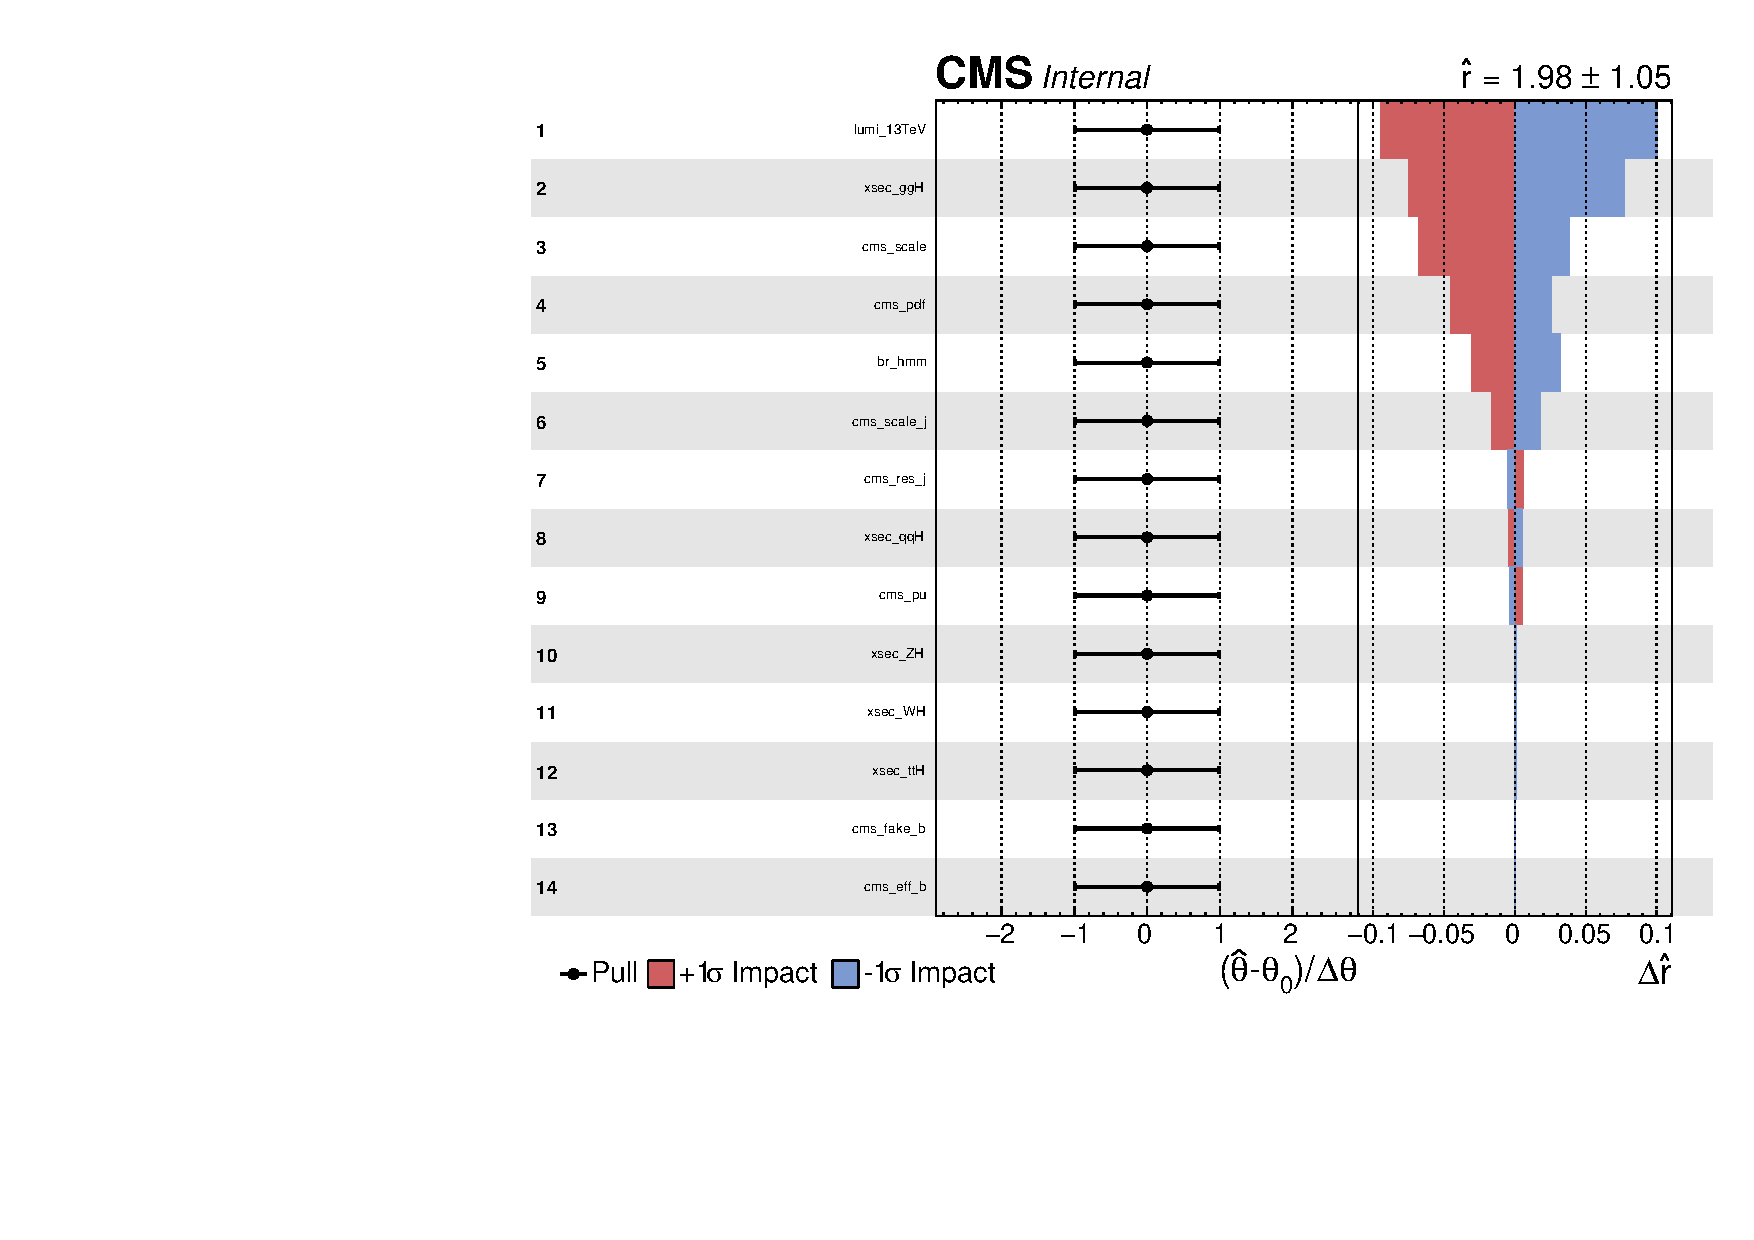
\includegraphics[width=0.631\textwidth]{figures/sig_syst/impacts.pdf}
%     \caption{Impact plots derived from the Asimov dataset.}
%     \label{fig:impacts}
% \end{figure}

% \section{Background systematic uncertainties}
% \label{bkg_syst}

% \subsection{Background fit function bias}
% As presented in Sec.~\ref{bkg_model} we identified two classes of models to fit the background
% dimuon mass spectrum, physics
% motivated models and general purpose series able to describle any smoothly falling
% functional forms (polynomials, sum of exponentials).

% The number of fit families considered in estimating the bias induced by the choice
% of the background fit function is constrained using the F-Test method at 95\% CL.

% The background fit functions are normalised to the data and 1000
% signal plus background toys were generated with the signal model and
% a certain background model. The obtained dimuon toy mass distribution
% is fit the signal plus background model where the background model
% can be any of the functional forms selected with the F-test. The obtained signal strength
% is compared with the injected one, here set to 1, and devided by the obtained signal strength
% error. The median is used to quote the background fit function bias.

% Two complete sets of bias scans in all categories at 125~GeV were conducted with independent
% toys and bias machinery. These are summarised in Appendix~\ref{app:Bias}.
% %The results for our most sensitive category of events are shown in Fig.~\ref{fig:cat12bias}.
% The baseline background model is the perturbed
% exponential times Breit-Wigner (``BWZRedux'').  The two sets of bias scans
% are checked explicitly for agreement in the BWZReduz bias against Bernstein
% polynomials and a sum of exponentials, with orders determined by the F-test.
% The bias vs. Bernstein is indicated by the purple box, and sum of exponentials
% by a black box, in the plots.

% In the end, we see that the two sets of bias scans agree quite well for most
% categories and pairs of fit vs. reference functions.  Some disagreements may
% be due to different orders of Bernstein polynomials being chosen by the F-tests.
% In c10, c8, c7, c5, c3, and c2, the Bernstein polynomial is biased against every
% other function, and every other function is biased against the Bernstein polynomial.
% This indicates that the Bernsteins do not characterize the data well in these
% categories, so they are excluded from consideration as reference functions.
% In c10 and c5, the BWZRedux bias against all other functions is less than 25\%.
% In c8, c7, and c3, a function formed of the BWZRedux plus a linear term has a
% bias of less than 25\% against all other functions, including the sum of exponentials.
% Categories c12, c11, c6, c4, and c1 all have at least one fit function with bias
% less than 20\% against all other functions.  Often this least-biased fit function
% is a Bernstein, while all the other fit functions are biased against the Bernstein.
% The BWZRedux function in category c9 has a 30 to 50\% bias against the Bernstein
% polynomial, and in c0 has 30 to 60\% bias against the sum of exponentials.

% Only in few categories will need explicit systematic uncertainties to parameterize
% the the bias due to choice of fit.  In most of these categories the bias is small,
% so the impact on the final limit is expected to be negligible.

%\begin{figure}
%  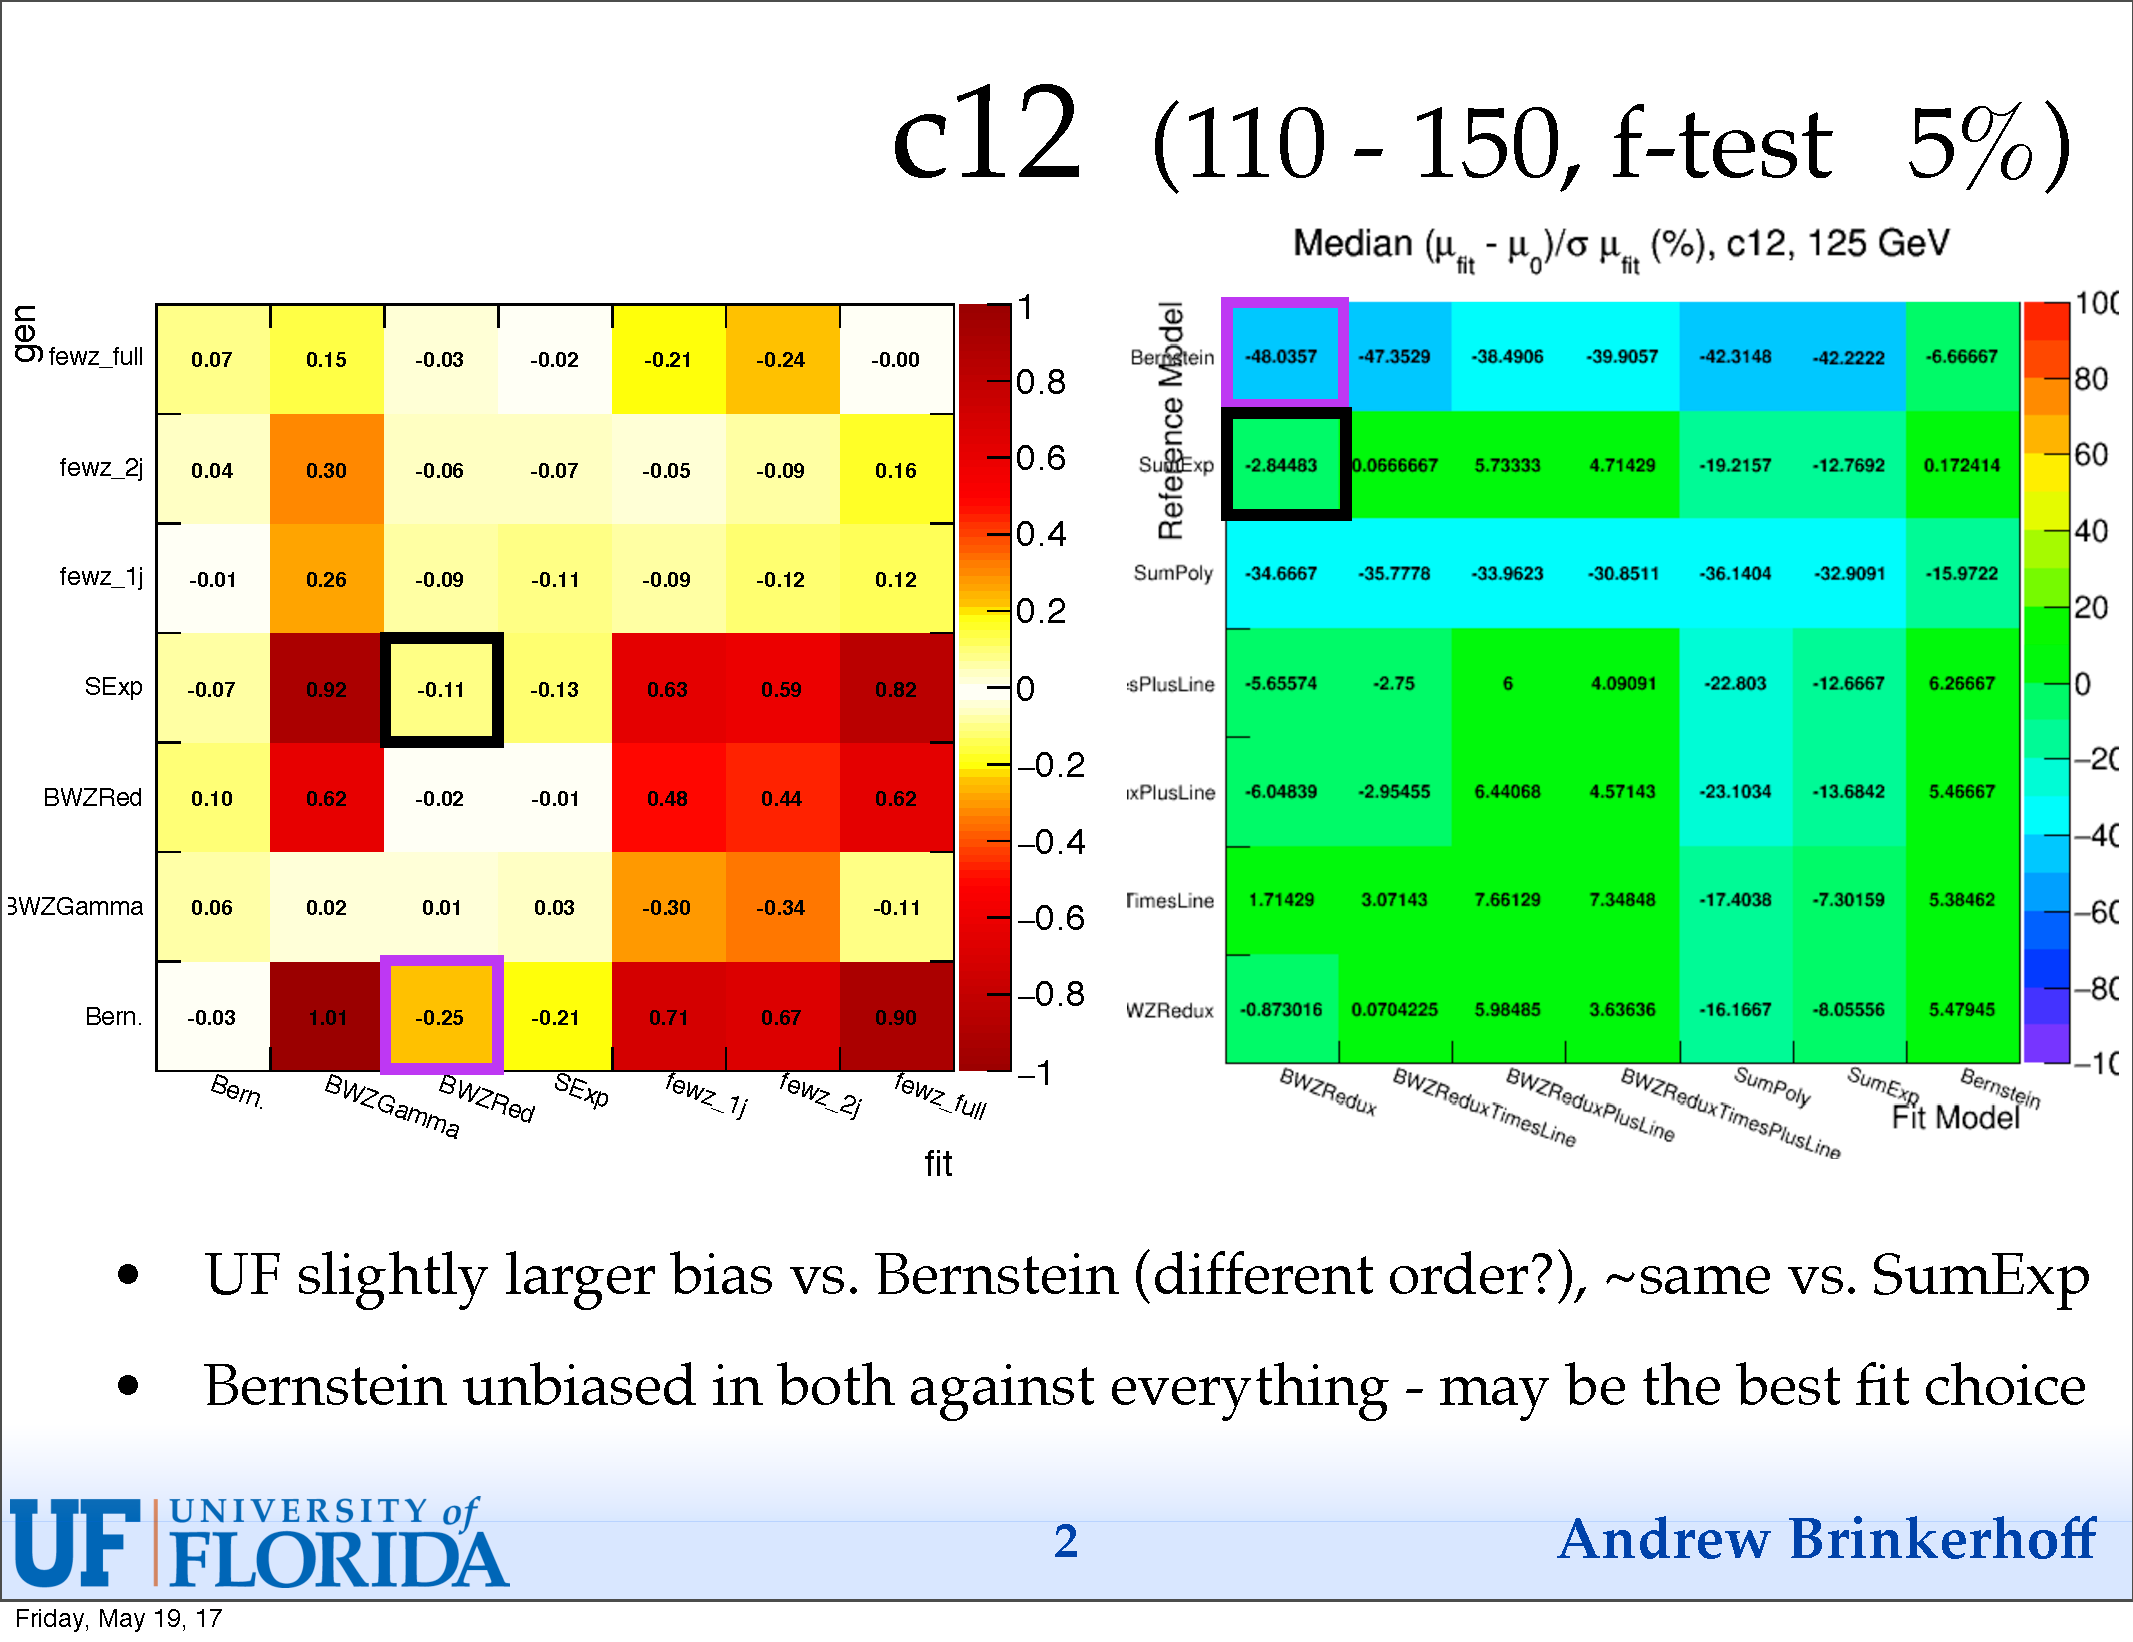
\includegraphics[width=0.8\textwidth]{figures/appendix_bias/UF_MIT_p1.pdf}
%  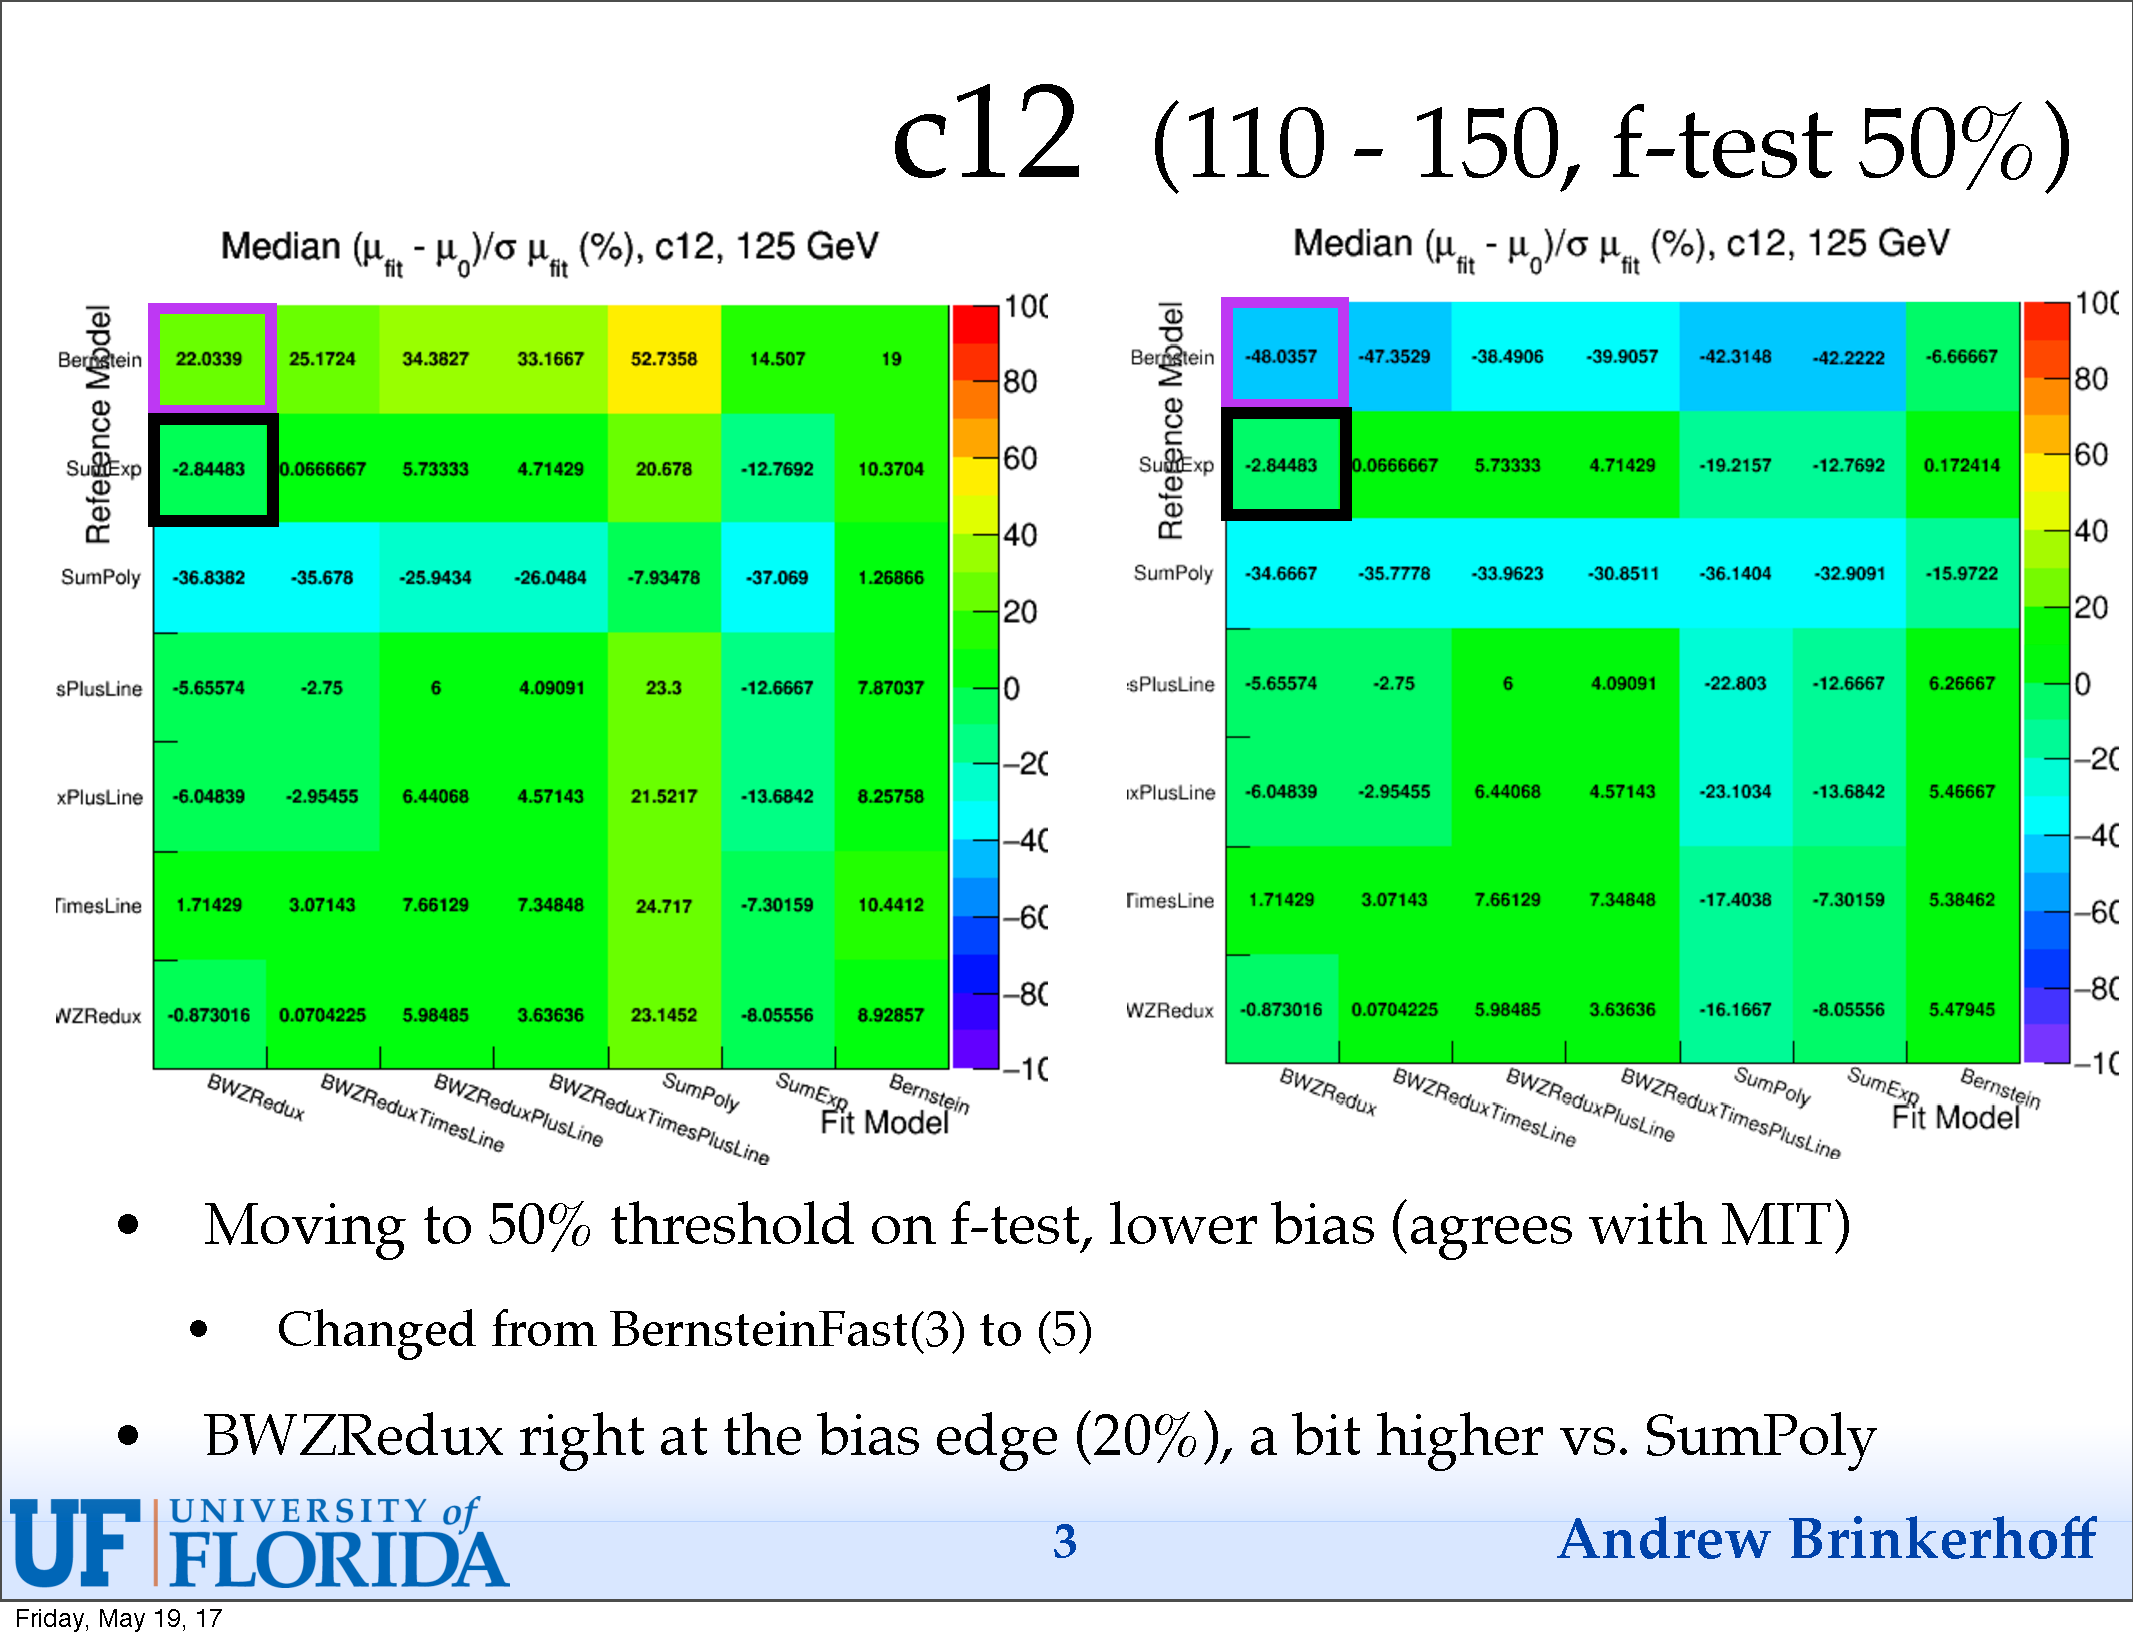
\includegraphics[width=0.8\textwidth]{figures/appendix_bias/UF_MIT_p2.pdf}
%  \label{fig:cat12bias}
%  \caption{The background fit function bias scan for the category 12 performed by MIT (left) and UF (right).}
%\end{figure}


%\subsection{Discrete profile method -- ``Envelope''}


